% Springer LNCS template (Overleaf: "Springer Lecture Notes in Computer Science").
% Upload results/feature_importance.png and results_balanced/confusion_matrix.png
% into the Overleaf project (keep the same folder names, or edit the paths below).
\documentclass[runningheads]{llncs}

\usepackage[T1]{fontenc}
\usepackage{graphicx}
\usepackage{booktabs}
\usepackage{amsmath}
\usepackage{xcolor}
\usepackage[hidelinks]{hyperref}

% Anything shown in red is a placeholder you must fill in before submitting.
\newcommand{\todo}[1]{\textcolor{red}{\textbf{[#1]}}}

\begin{document}

\title{Lightweight Machine Learning for Detecting Attacks on IoT Networks: Handling Class Imbalance and Model Size}
\titlerunning{Lightweight ML Intrusion Detection for IoT}

\author{Smridhi}
\authorrunning{Smridhi}
\institute{Thapar Institute of Engineering and Technology, Patiala, Punjab, India}

\maketitle

\begin{abstract}
The number of connected Internet of Things (IoT) devices keeps growing, yet many of them are weakly protected, rarely patched and easy to recruit into botnets. Network intrusion detection tools used in practice, such as Snort and Suricata, rely mainly on hand-written signatures. They need continuous rule maintenance and are built for gateways and servers, not for constrained environments. Machine-learning-based detectors are a promising alternative, but many published studies report only overall accuracy on heavily imbalanced data and ignore the memory and time cost of the model. This article studies these two issues on the public CIC IoT Attack Dataset 2023 (CICIoT2023). We train six classifiers on flow-level features (Logistic Regression, Decision Tree, three Random Forest variants and XGBoost), apply random-forest-based feature selection, and compare standard training with class-weighted training. On a test set of about 60,000 flows in which only 2.3\% of the flows are benign, all models reach 98.7--99.2\% accuracy in the standard setting, but the benign-class recall is only 69--82\%. Class weighting raises benign recall to 99.1\% for a 15-feature XGBoost model of only 179~KB, at the cost of about one percentage point of attack recall. This model is about 91 times smaller than the full Random Forest (16.3~MB). We discuss the trade-offs and limitations, and we release the code publicly.
\keywords{IoT security \and intrusion detection \and machine learning \and class imbalance \and CICIoT2023 \and lightweight models.}
\end{abstract}

%-------------------------------------------------------------------
\section{Introduction}
\label{sec:intro}

The Internet of Things (IoT) connects cameras, sensors, smart plugs, routers and many other devices to the Internet. Many of these devices have limited processing power and memory, ship with default credentials, and receive few or no security updates. Attackers exploit this: the Mirai botnet showed that large numbers of compromised devices can be turned into a platform for large-scale distributed denial-of-service (DDoS) attacks~\cite{antonakakis2017,kolias2017}. For this reason, the security of IoT networks is a practical problem in domains such as smart homes, healthcare, agriculture and industry.

\paragraph{Problem.} The tools most widely used to watch network traffic are network intrusion detection systems (NIDS) such as Snort~\cite{roesch1999}, Suricata~\cite{suricata} and Zeek~\cite{paxson1999}. They work mainly by matching traffic against signatures and rules written by experts. In IoT settings this has three drawbacks: rules must be written and updated for every new attack family or variant, so a new variant can pass unnoticed until a rule exists; the tools are designed for gateways, servers or appliances, not for constrained deployments; and IoT traffic is so diverse that writing rules for every device type is expensive.

Machine learning (ML) can learn to separate normal from malicious traffic from labelled examples and can be retrained when new data arrives. ML-based detection has its own weaknesses, however. Sommer and Paxson~\cite{sommer2010} explained why it is hard to use in operations, and Arp et al.~\cite{arp2022} listed common pitfalls in security-related ML studies, including inappropriate performance measures and the base-rate fallacy. Two issues are especially visible in the IoT literature: (i)~intrusion datasets are strongly imbalanced, so overall accuracy hides poor performance on the minority class; and (ii)~the memory and time cost of the model is often not reported, although it decides whether the model can run close to the device.

\paragraph{Contributions.} This article makes the following contributions.
\begin{enumerate}
\item We build a reproducible experimental pipeline on the public CICIoT2023 dataset~\cite{neto2023} that compares six classifiers on flow-level features.
\item We evaluate the models with imbalance-aware measures (macro F1, balanced accuracy, and per-class recall) in addition to accuracy, and we show how much overall accuracy can hide.
\item We compare standard training with class-weighted training and quantify the trade-off between false alarms on benign traffic and missed attacks.
\item We report model size and inference time, and we show that a 15-feature XGBoost model of 179~KB gives a good balance between detection quality and resource cost.
\item We release all code in a public repository: https://github.com/smridhigarg/iot-ids-lightweight-ml.
\end{enumerate}

%-------------------------------------------------------------------
\section{Literature Review}
\label{sec:lit}

\subsection{Signature-based network intrusion detection tools}
Snort~\cite{roesch1999} and Suricata~\cite{suricata} are open-source engines that inspect traffic and compare it with a rule set; Suricata also offers intrusion prevention and uses a rule language similar to Snort's. Zeek~\cite{paxson1999} instead turns traffic into events that analyst-written scripts react to. Commercial intrusion detection and prevention appliances follow the same general idea with vendor-maintained signature feeds. These tools are reliable when good rules exist. Their main limitation, which motivates this work, is the dependence on human-written rules: they are strong against known patterns, weaker against new variants, and need continuous maintenance.

\subsection{Machine learning for network intrusion detection}
Buczak and Guven~\cite{buczak2016} survey data-mining and ML methods for intrusion detection. Sommer and Paxson~\cite{sommer2010} argue that intrusion detection differs from other ML applications because errors are costly, traffic is very diverse and evaluation is difficult, which explains why ML detectors are rarely used in production. For IoT, Meidan et al.~\cite{meidan2018} proposed N-BaIoT, which applies deep autoencoders to traffic from IoT devices to detect botnet attacks, and Mirsky et al.~\cite{mirsky2018} proposed Kitsune, an online ensemble of autoencoders designed to be light enough to run in a network device. Tree-based models such as Random Forest~\cite{breiman2001} and XGBoost~\cite{chen2016} are popular for tabular flow features because they train quickly and often perform very well, but their size varies strongly with the number and depth of trees, which is why we measure it.

\subsection{Datasets and class imbalance}
UNSW-NB15~\cite{moustafa2015} and CICIDS2017~\cite{sharafaldin2018} are widely used general network datasets, but they were not collected in an IoT topology. CICIoT2023~\cite{neto2023} was built with 105 IoT devices, and its attacks are executed by malicious IoT devices against other IoT devices. It covers 33 attacks in seven categories (DDoS, DoS, reconnaissance, web-based, brute force, spoofing and Mirai) plus benign traffic, and is provided as packet captures and as flow-feature CSV files~\cite{cic}; we use the CSV version. Intrusion datasets are rarely balanced: here the attack classes dominate by design, whereas real networks carry mostly benign traffic. He and Garcia~\cite{he2009} survey methods for learning from imbalanced data, including resampling (for example SMOTE~\cite{chawla2002}) and cost-sensitive learning, which keeps the data unchanged and gives minority-class errors a higher weight; we use the latter. Arp et al.~\cite{arp2022} warn that accuracy-only reporting on imbalanced data and ignoring base rates are common pitfalls, so we report per-class recall, macro F1 and balanced accuracy.

\subsection{Research gap}
Table~\ref{tab:compare} summarises how this work relates to signature-based tools. From the review we identify the following gaps, which this article addresses.
\begin{itemize}
\item \textbf{Gap 1 -- Rule dependence.} Signature tools need constant manual rule maintenance. A model learned from flow features can be retrained on new labelled data instead.
\item \textbf{Gap 2 -- Misleading metrics.} Many ML studies report overall accuracy only. On a dataset with 98\% attacks, such a metric hides how often benign traffic is misclassified.
\item \textbf{Gap 3 -- Resource cost is not reported.} Model size and inference time are often missing, although they decide whether a detector can run near the devices.
\end{itemize}

\begin{table}[t]
\caption{Qualitative comparison between signature-based NIDS and the approach of this article. Resource figures for the signature tools were not measured in this study.}
\label{tab:compare}
\centering
\small
\begin{tabular}{p{2.4cm}p{4.0cm}p{4.3cm}}
\toprule
Property & Signature-based NIDS (Snort, Suricata) & This work (learned model) \\
\midrule
Detection basis & Hand-written rules and signatures & Patterns learned from labelled flow features \\
Keeping up with new attacks & New or updated rules are needed & Retraining on new labelled data \\
Input & Packet headers and payload & Flow-level statistics (39 features) \\
Footprint & Not measured here & 179~KB model (XGBoost, 15 features) \\
Main weakness & Misses variants without a rule & Needs labelled data; sensitive to class imbalance \\
\bottomrule
\end{tabular}
\end{table}

%-------------------------------------------------------------------
\section{Technology Used and Methodology}
\label{sec:method}

\subsection{Overview}
The pipeline has five steps: flow records are loaded and cleaned, split into training and test sets, a feature subset is selected from the training data only, six models are trained under two settings (standard and class-weighted), and each model is evaluated for detection quality and resource cost. The code is in the public repository (Section~\ref{sec:conclusion}).


\subsection{Dataset and preprocessing}
We use the flow-feature CSV files of CICIoT2023~\cite{neto2023}. We sampled rows evenly from several of the merged CSV part files (listed in the repository), for a total of 199,995 flows after cleaning (target 200,000). We cleaned the data by keeping numeric columns only, replacing infinite values by missing values, dropping rows with missing values, and removing constant columns. This leaves 39 input features, for example header length, protocol type, time-to-live, flow rate, TCP flag indicators, flag counts and protocol indicators such as HTTP, HTTPS, DNS, Telnet and SMTP. We then converted the task to a binary one: every flow whose label is benign is class 0, and every other flow is class 1 (attack). The resulting data contains 195,379 attack flows and only 4,616 benign flows, so benign flows are 2.3\% of the data. The data was split with a stratified 70/30 train/test split (random seed 42), which gives about 140,000 training flows and about 60,000 test flows, of which about 1,385 are benign.

\subsection{Feature selection}
To reduce the model size and the inference cost we rank the features with the importance scores of a Random Forest (50 trees) trained on the training set only, and we keep the 15 most important features for four of the six models. The test set is never used for this step.

\subsection{Classifiers}
We compare six classifiers implemented with scikit-learn~\cite{pedregosa2011} and XGBoost~\cite{chen2016}: Logistic Regression (LR) on all 39 standardised features; a Decision Tree (DT) with default settings; a Random Forest with 100 trees on all features (RF-all); the same forest on the top-15 features (RF-15); a small Random Forest on the top-15 features with 30 trees of maximum depth 12 (RF-small); and XGBoost with 100 trees of maximum depth 6 on the top-15 features (XGB-15).

\subsection{Handling class imbalance}
We run all experiments twice. In the \emph{standard} setting, every training flow has the same weight. In the \emph{class-weighted} setting, errors on the minority (benign) class receive a higher weight: for LR, DT and the Random Forests we use the ``balanced'' class weights of scikit-learn, which are inversely proportional to class frequencies, and for XGBoost we set \texttt{scale\_pos\_weight} to the ratio of benign to attack training flows ($\approx$0.024). The data itself is not changed (no resampling).

\subsection{Evaluation measures}
The recall of a class is the share of its flows that are correctly recognised. We report accuracy; \textbf{benign recall}, where $1-\text{benign recall}$ is the false alarm rate on normal traffic; \textbf{attack recall}; \textbf{balanced accuracy}, the mean of the two recalls; \textbf{macro F1}, the unweighted mean of the F1 scores of the two classes; \textbf{model size}, the size in KB of the model serialised with \texttt{joblib}; and \textbf{inference time} in milliseconds per 1,000 test flows.

\subsection{Implementation}
The code is written in Python~3 (scikit-learn 1.9.1, XGBoost 3.4.1, pandas 3.1.1, NumPy 2.5.5) and was run on a standard Windows laptop. One command runs the whole pipeline and writes the results to CSV files and figures.

%-------------------------------------------------------------------
\section{Experimental Results}
\label{sec:results}

\subsection{Standard training}
Table~\ref{tab:standard} shows the results when all flows have equal weight. The accuracy of all six models is between 98.7\% and 99.2\%, which looks excellent. The other columns show a different picture: the benign recall lies between 69.1\% (LR) and 81.7\% (RF-all), so between about 18\% and 31\% of the normal flows are wrongly flagged as attacks. Macro F1 (0.85--0.91) and balanced accuracy (0.84--0.91) are much lower than accuracy. The reason is simple: because 97.7\% of the flows are attacks, a model that always answers ``attack'' would already reach 97.7\% accuracy, so differences of a few tenths of a percent in accuracy say little about the minority class.

\begin{table}[t]
\caption{Results with standard training (no class weights). Recall values are for the benign and attack classes; Size is the serialised model size; Inf.\ is inference time in ms per 1,000 flows.}
\label{tab:standard}
\centering
\scriptsize
\setlength{\tabcolsep}{3pt}
\begin{tabular}{lccccccc}
\toprule
Model & Acc. & Macro F1 & Bal.\ acc. & Benign R. & Attack R. & Size (KB) & Inf. \\
\midrule
LR & 0.9869 & 0.8512 & 0.8424 & 0.6910 & 0.9939 & 3.2 & 0.661 \\
DT & 0.9890 & 0.8789 & 0.8826 & 0.7711 & 0.9941 & 157.4 & 0.308 \\
RF-all & 0.9919 & 0.9094 & 0.9067 & 0.8173 & 0.9960 & 15,825.2 & 2.745 \\
RF-15 & 0.9910 & 0.9001 & 0.9002 & 0.8051 & 0.9954 & 15,251.6 & 2.168 \\
RF-small & 0.9909 & 0.8983 & 0.8973 & 0.7993 & 0.9954 & 1,565.1 & 1.125 \\
XGB-15 & 0.9903 & 0.8922 & 0.8918 & 0.7884 & 0.9951 & 256.0 & 1.185 \\
\bottomrule
\end{tabular}
\end{table}

\subsection{Class-weighted training}
Table~\ref{tab:weighted} shows the same experiment with class weights. The effect depends on the model. For LR, RF-small and XGB-15, benign recall increases to 99.9\%, 99.3\% and 99.1\%, respectively, and balanced accuracy increases to about 0.988 for the three models. For the large Random Forests the gain is smaller (benign recall of 93.0\% for RF-all and 92.6\% for RF-15). The Decision Tree does not change at all (benign recall 77.1\%), which is expected for a tree that is grown until its leaves are pure, since class weights have little influence on such a tree.

The gain on benign traffic has a price. Attack recall decreases for the models that benefit most: from 99.5\% to 98.5\% for XGB-15, from 99.5\% to 98.4\% for RF-small, and from 99.4\% to 97.7\% for LR. Overall accuracy therefore decreases slightly (for example from 99.0\% to 98.5\% for XGB-15), and macro F1 even decreases for these models. A back-of-envelope calculation from the recalls and the class counts of the test set indicates that this is because the benign class then receives many attack flows that were classified as benign: the precision for the benign class falls to roughly 0.5--0.6 for LR, RF-small and XGB-15. In other words, class weighting moves errors from one side to the other, and it is a trade-off that has to be chosen according to the deployment.

\begin{table}[t]
\caption{Results with class-weighted training. Same columns as Table~\ref{tab:standard}.}
\label{tab:weighted}
\centering
\scriptsize
\setlength{\tabcolsep}{3pt}
\begin{tabular}{lccccccc}
\toprule
Model & Acc. & Macro F1 & Bal.\ acc. & Benign R. & Attack R. & Size (KB) & Inf. \\
\midrule
LR & 0.9770 & 0.8279 & 0.9879 & 0.9993 & 0.9765 & 3.2 & 0.472 \\
DT & 0.9896 & 0.8843 & 0.8829 & 0.7711 & 0.9948 & 220.9 & 0.285 \\
RF-all & 0.9911 & 0.9116 & 0.9612 & 0.9300 & 0.9925 & 16,342.4 & 3.000 \\
RF-15 & 0.9903 & 0.9047 & 0.9587 & 0.9256 & 0.9918 & 15,948.1 & 2.142 \\
RF-small & 0.9841 & 0.8673 & 0.9884 & 0.9928 & 0.9839 & 1,677.3 & 0.915 \\
XGB-15 & 0.9851 & 0.8730 & 0.9878 & 0.9906 & 0.9849 & 178.7 & 1.329 \\
\bottomrule
\end{tabular}
\end{table}

\subsection{Model size and inference time}
The memory footprint differs by more than three orders of magnitude, from 3.2~KB (LR) to 16.3~MB (RF-all, class-weighted). The XGB-15 model needs only 178.7~KB, which is about 91 times less than RF-all, and its inference time (1.33~ms per 1,000 flows) is about 2.3 times lower than that of RF-all (3.00~ms). RF-small is about 10 times smaller than RF-all (1.6~MB) and needs 0.92~ms per 1,000 flows. Reducing the features from 39 to 15 alone did not reduce the size of the Random Forest noticeably (15.9~MB versus 16.3~MB); the savings come from using fewer and shallower trees, or from boosting with shallow trees. Fig.~\ref{fig:fi} shows the feature ranking used for the selection.

\begin{figure}[t]
\centering
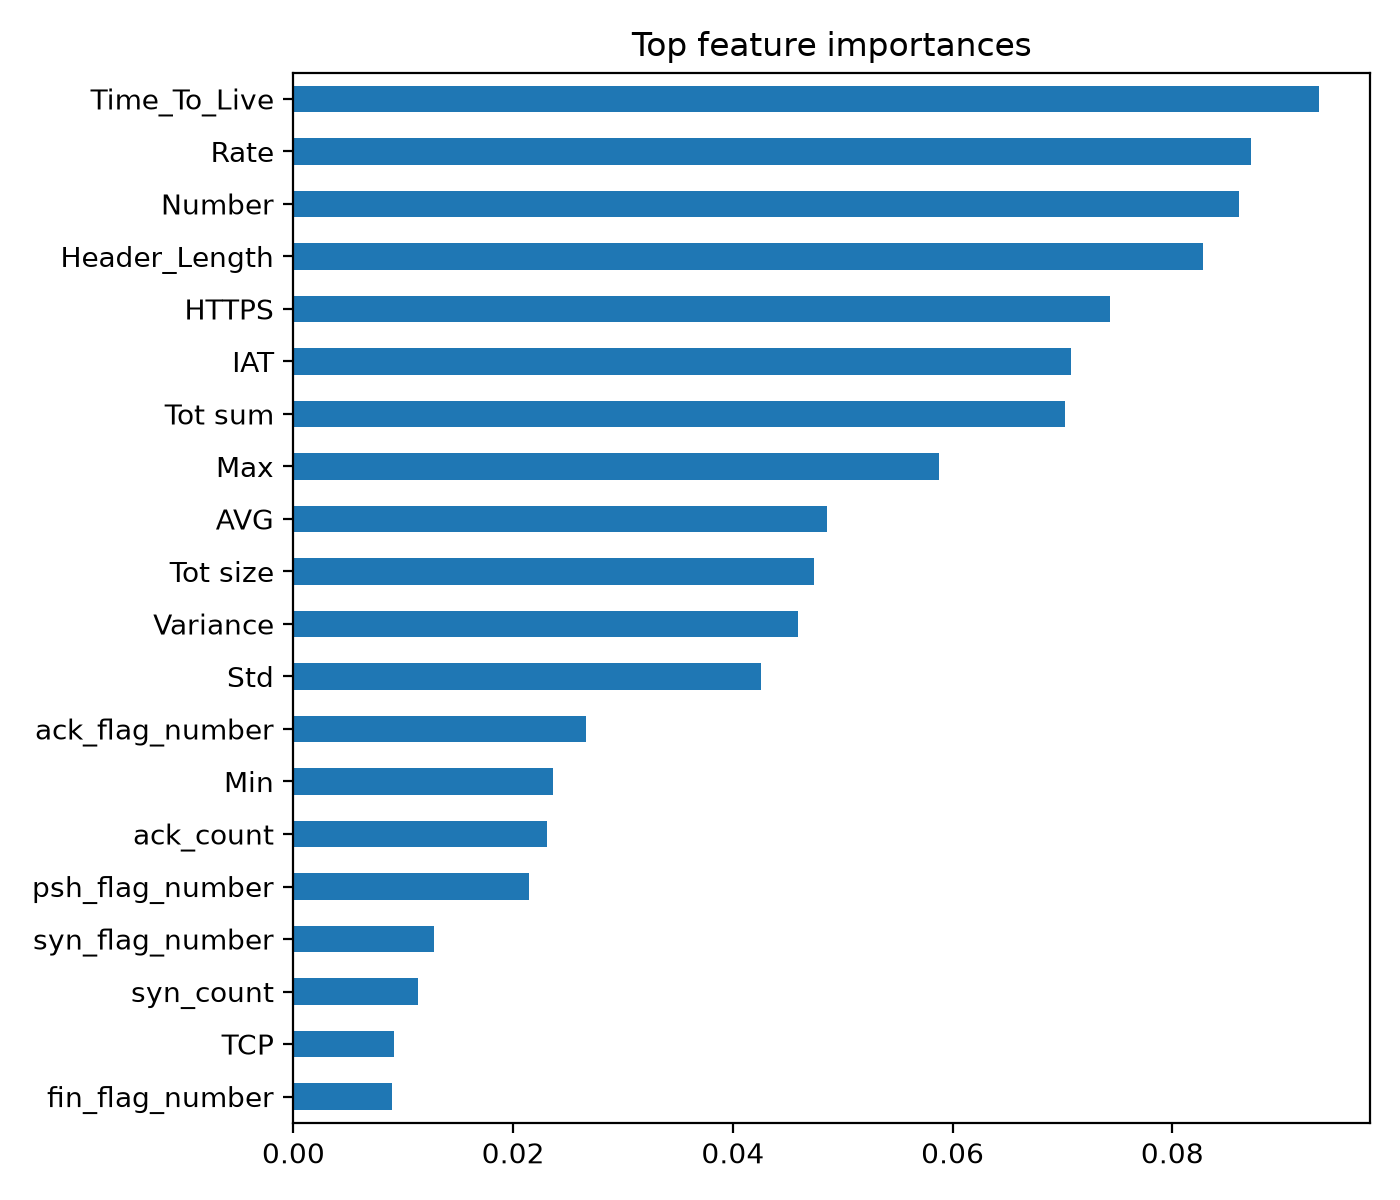
\includegraphics[width=0.55\textwidth]{results/feature_importance.png}
\caption{Feature importance (top 20) from the Random Forest ranking used for feature selection.}
\label{fig:fi}
\end{figure}

\begin{figure}[t]
\centering
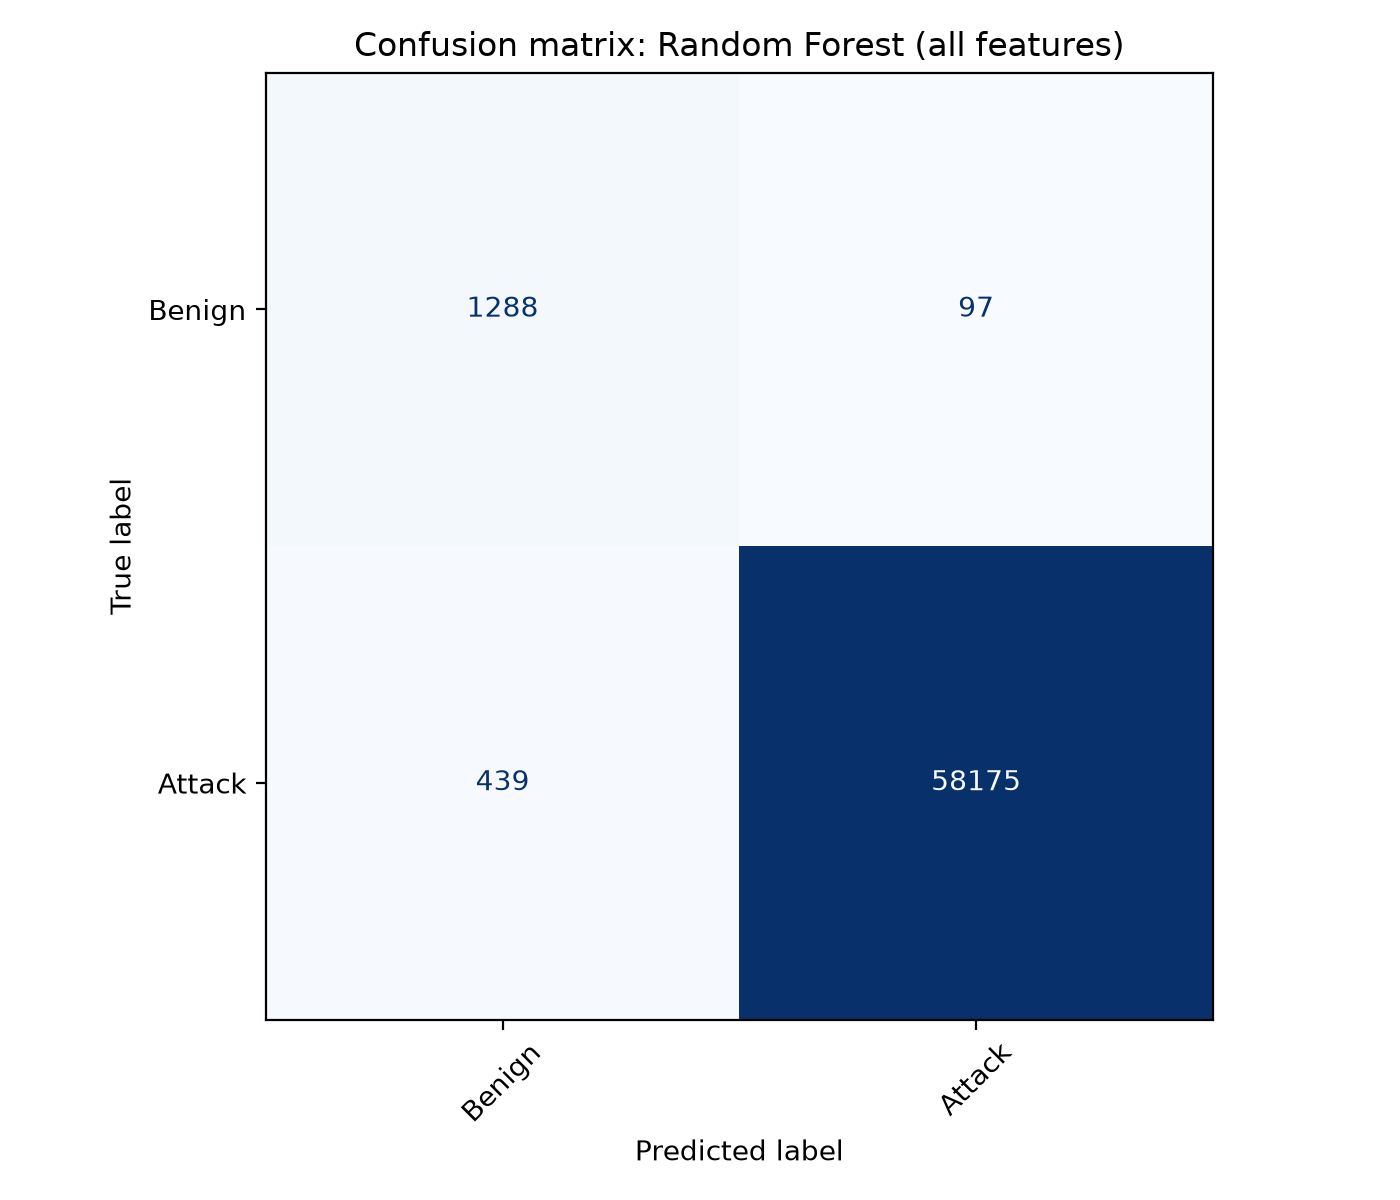
\includegraphics[width=0.5\textwidth]{results_balanced/confusion_matrix.png}
\caption{Confusion matrix on the test set for the class-weighted experiment (model with the best weighted F1, as selected by the script).}
\label{fig:cm}
\end{figure}

\subsection{Choosing a model}
No model is best on every measure. RF-all has the highest macro F1 (0.912) but is large. XGB-15 and RF-small combine about 99\% benign recall with about 98.4--98.5\% attack recall at 179~KB and 1.6~MB. LR has the highest benign recall (99.9\%) and a 3~KB model, but it misses the most attacks (2.4\%).

%-------------------------------------------------------------------
\section{Discussion and Limitations}
\label{sec:discussion}

\paragraph{Relation to existing tools.} The comparison with signature-based NIDS here is qualitative (Table~\ref{tab:compare}): we did not run Snort or Suricata on the data, so we make no claim about their detection rate or resource use. Our experiments show that a learned detector on flow features can reach about 99\% recall on both classes with a model under 200~KB, and that this is only visible when imbalance-aware measures are reported.

\paragraph{Meaning for deployment.} Real networks carry mostly benign traffic, so the false alarm rate on benign flows ($1-$benign recall) is the more relevant number. With standard training it is 21\% for XGB-15, which would be unusable; with class weights it falls to about 0.9\%. Because the attack base rate in real traffic is far lower than in this dataset, even this rate can create many alerts~\cite{arp2022}, so a threshold tuned on realistic traffic would be needed before deployment.

\paragraph{Limitations.} (i)~We used one random split and one run per setting, without cross-validation or confidence intervals, on a subset of the dataset. (ii)~Flows from the same session can be very similar, so a random split may be optimistic compared with unseen traffic. (iii)~Only one dataset was used and cross-dataset generalisation was not tested. (iv)~Timings come from one laptop CPU, with parallel prediction for the Random Forests, so they show the relative order of the models but are not measurements on IoT hardware. (v)~The task was reduced to benign versus attack, and the 33 attack types were not evaluated separately. (vi)~Signature-based tools were not benchmarked directly.

%-------------------------------------------------------------------
\section{Conclusion and Future Work}
\label{sec:conclusion}

We studied intrusion detection for IoT networks with lightweight ML models on CICIoT2023, with attention to two issues that are often neglected: class imbalance and resource cost. In the data used here, accuracy of about 99\% hid a benign recall of only 69--82\%. Class-weighted training raised benign recall to about 99\% for compact models, with a loss of about one percentage point of attack recall, and a 15-feature XGBoost model of 179~KB achieved a good balance. Reporting per-class recall, balanced accuracy and model size gives a more honest picture than accuracy alone.

Future work includes evaluating on all 33 attack types, cross-validation and cross-dataset tests, a direct benchmark against Snort and Suricata, resampling methods such as SMOTE~\cite{chawla2002} compared with class weighting, threshold tuning for realistic traffic ratios, and measuring the models on real IoT hardware such as a Raspberry Pi.

\paragraph{Code availability.} The source code, instructions and result files are available at https://github.com/smridhigarg/iot-ids-lightweight-ml. The dataset is publicly available from the Canadian Institute for Cybersecurity~\cite{cic} and is not included in the repository.

\begin{thebibliography}{9}
\bibitem{antonakakis2017} Antonakakis, M., et al.: Understanding the Mirai botnet. In: 26th USENIX Security Symposium, pp.~1093--1110 (2017)
\bibitem{kolias2017} Kolias, C., Kambourakis, G., Stavrou, A., Voas, J.: DDoS in the IoT: Mirai and other botnets. Computer \textbf{50}(7), 80--84 (2017)
\bibitem{roesch1999} Roesch, M.: Snort: Lightweight intrusion detection for networks. In: Proc.\ 13th USENIX Large Installation System Administration Conference (LISA), pp.~229--238 (1999)
\bibitem{suricata} Open Information Security Foundation: Suricata. \url{https://suricata.io}, last accessed 2026
\bibitem{paxson1999} Paxson, V.: Bro: A system for detecting network intruders in real-time. Computer Networks \textbf{31}(23--24), 2435--2463 (1999)
\bibitem{sommer2010} Sommer, R., Paxson, V.: Outside the closed world: On using machine learning for network intrusion detection. In: IEEE Symposium on Security and Privacy, pp.~305--316 (2010)
\bibitem{arp2022} Arp, D., et al.: Dos and don'ts of machine learning in computer security. In: 31st USENIX Security Symposium (2022)
\bibitem{neto2023} Neto, E.C.P., Dadkhah, S., Ferreira, R., Zohourian, A., Lu, R., Ghorbani, A.A.: CICIoT2023: A real-time dataset and benchmark for large-scale attacks in IoT environment. Sensors \textbf{23}(13), 5941 (2023). \url{https://doi.org/10.3390/s23135941}
\bibitem{buczak2016} Buczak, A.L., Guven, E.: A survey of data mining and machine learning methods for cyber security intrusion detection. IEEE Commun.\ Surveys Tuts.\ \textbf{18}(2), 1153--1176 (2016)
\bibitem{meidan2018} Meidan, Y., et al.: N-BaIoT: Network-based detection of IoT botnet attacks using deep autoencoders. IEEE Pervasive Comput.\ \textbf{17}(3), 12--22 (2018)
\bibitem{mirsky2018} Mirsky, Y., Doitshman, T., Elovici, Y., Shabtai, A.: Kitsune: An ensemble of autoencoders for online network intrusion detection. In: Network and Distributed System Security Symposium (NDSS) (2018)
\bibitem{breiman2001} Breiman, L.: Random forests. Machine Learning \textbf{45}(1), 5--32 (2001)
\bibitem{chen2016} Chen, T., Guestrin, C.: XGBoost: A scalable tree boosting system. In: Proc.\ 22nd ACM SIGKDD Int.\ Conf.\ Knowledge Discovery and Data Mining, pp.~785--794 (2016)
\bibitem{moustafa2015} Moustafa, N., Slay, J.: UNSW-NB15: A comprehensive data set for network intrusion detection systems. In: Military Communications and Information Systems Conference (MilCIS), pp.~1--6. IEEE (2015)
\bibitem{sharafaldin2018} Sharafaldin, I., Lashkari, A.H., Ghorbani, A.A.: Toward generating a new intrusion detection dataset and intrusion traffic characterization. In: Proc.\ 4th Int.\ Conf.\ Information Systems Security and Privacy (ICISSP), pp.~108--116 (2018)
\bibitem{cic} Canadian Institute for Cybersecurity: CIC IoT dataset 2023. \url{https://www.unb.ca/cic/datasets/iotdataset-2023.html}, last accessed 2026
\bibitem{he2009} He, H., Garcia, E.A.: Learning from imbalanced data. IEEE Trans.\ Knowl.\ Data Eng.\ \textbf{21}(9), 1263--1284 (2009)
\bibitem{chawla2002} Chawla, N.V., Bowyer, K.W., Hall, L.O., Kegelmeyer, W.P.: SMOTE: Synthetic minority over-sampling technique. J.\ Artif.\ Intell.\ Res.\ \textbf{16}, 321--357 (2002)
\bibitem{pedregosa2011} Pedregosa, F., et al.: Scikit-learn: Machine learning in Python. J.\ Mach.\ Learn.\ Res.\ \textbf{12}, 2825--2830 (2011)
\end{thebibliography}

\end{document}
